\documentclass[]{elsarticle} %review=doublespace preprint=single 5p=2 column
%%% Begin My package additions %%%%%%%%%%%%%%%%%%%
\usepackage[hyphens]{url}

  \journal{An awesome journal} % Sets Journal name


\usepackage{lineno} % add
\providecommand{\tightlist}{%
  \setlength{\itemsep}{0pt}\setlength{\parskip}{0pt}}

\usepackage{graphicx}
\usepackage{booktabs} % book-quality tables
%%%%%%%%%%%%%%%% end my additions to header

\usepackage[T1]{fontenc}
\usepackage{lmodern}
\usepackage{amssymb,amsmath}
\usepackage{ifxetex,ifluatex}
\usepackage{fixltx2e} % provides \textsubscript
% use upquote if available, for straight quotes in verbatim environments
\IfFileExists{upquote.sty}{\usepackage{upquote}}{}
\ifnum 0\ifxetex 1\fi\ifluatex 1\fi=0 % if pdftex
  \usepackage[utf8]{inputenc}
\else % if luatex or xelatex
  \usepackage{fontspec}
  \ifxetex
    \usepackage{xltxtra,xunicode}
  \fi
  \defaultfontfeatures{Mapping=tex-text,Scale=MatchLowercase}
  \newcommand{\euro}{€}
\fi
% use microtype if available
\IfFileExists{microtype.sty}{\usepackage{microtype}}{}
\bibliographystyle{elsarticle-harv}
\usepackage{graphicx}
% We will generate all images so they have a width \maxwidth. This means
% that they will get their normal width if they fit onto the page, but
% are scaled down if they would overflow the margins.
\makeatletter
\def\maxwidth{\ifdim\Gin@nat@width>\linewidth\linewidth
\else\Gin@nat@width\fi}
\makeatother
\let\Oldincludegraphics\includegraphics
\renewcommand{\includegraphics}[1]{\Oldincludegraphics[width=\maxwidth]{#1}}
\ifxetex
  \usepackage[setpagesize=false, % page size defined by xetex
              unicode=false, % unicode breaks when used with xetex
              xetex]{hyperref}
\else
  \usepackage[unicode=true]{hyperref}
\fi
\hypersetup{breaklinks=true,
            bookmarks=true,
            pdfauthor={},
            pdftitle={Short Paper},
            colorlinks=false,
            urlcolor=blue,
            linkcolor=magenta,
            pdfborder={0 0 0}}
\urlstyle{same}  % don't use monospace font for urls

\setcounter{secnumdepth}{0}
% Pandoc toggle for numbering sections (defaults to be off)
\setcounter{secnumdepth}{0}
% Pandoc header



\begin{document}
\begin{frontmatter}

  \title{Short Paper}
    \author[Some Institute of Technology]{Alice Anonymous\corref{c1}}
   \ead{alice@example.com} 
   \cortext[c1]{Corresponding Author}
    \author[Another University]{Bob Security}
   \ead{bob@example.com} 
  
      \address[Some Institute of Technology]{Department, Street, City, State, Zip}
    \address[Another University]{Department, Street, City, State, Zip}
  
  \begin{abstract}
  This is the abstract.
  
  It consists of two paragraphs.
  \end{abstract}
  
 \end{frontmatter}

\hypertarget{introduction}{%
\section{Introduction}\label{introduction}}

The economy of a nation is tied to its consumption of energy, since
every process of production requires energy as an input. However, the
strength of the relationship between the economy and the consumption of
energy varies. Some countries (e.g., Japan) were more successful than
others in terms of decoupling their productive processes from energy
after the oil shocks of the 1970s. This was achieved by increasing the
efficiency of production, so that the same output could be produced
using less energy, or in somewhat different terms, by improving their
energy intensity.

The relationship between economic output and energy consumption is of
interest at a time when the effects of a carbon-intense economy is
creating a heavy environmental burden. A relevant question is, what
countries are more energy-efficient, and can we learn from them. To
explore this question we will consider data on national energy use (in
barrels of oil per day), economic output (GDP), and \(CO_2\) emissions.

Figure \ref{fig:energy-to-gdp} is a scatterplot of energy consumption to
GPD. It can be seen that in general, greater economic output is
associated with greater consumption of energy. However, there are some
important differences. If we fit a regression line to this relationship,
the line would indicate the \emph{expected} economic output for a given
level of energy consumption. Points below the line would use more energy
for a lower level of economic output than expected, whereas points above
the line would represent greater economic output than expected, given
their energy consumption.

\begin{figure}
\centering
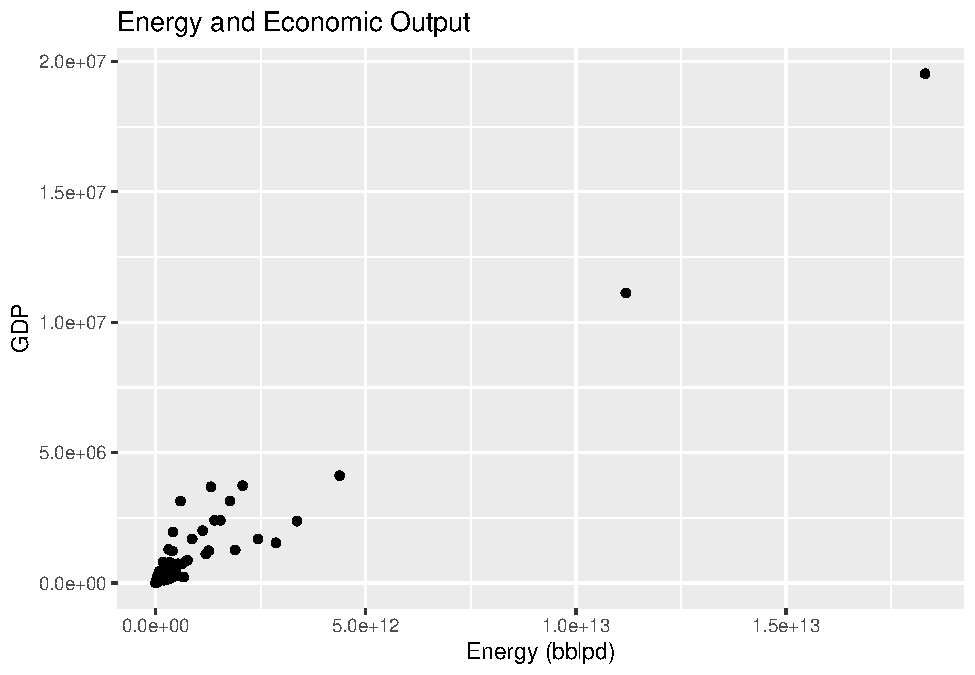
\includegraphics{Elsevier-Template_files/figure-latex/fig-energy-to-gdp-1.pdf}
\caption{\label{fig:energy-to-gdp} The relationship between energy
consumption and economic output by world countries}
\end{figure}

The regression line is estimated as follows: \[
GDP_i = \beta_0 + \beta_1\text{bblpd}_i + \epsilon_i
\]

This is a linear model and can be estimated using ordinary least
squares. The scatterplot of energy to GDP with this line is shown in
Figure \ref{fig:energy-to-gdp-with-line}. Clearly, some countries are
more efficient than others in that they can produce more with less
energy. The more a point deviates from the regression line, the more
efficient that economy is. It would be interesting to

\begin{figure}
\centering
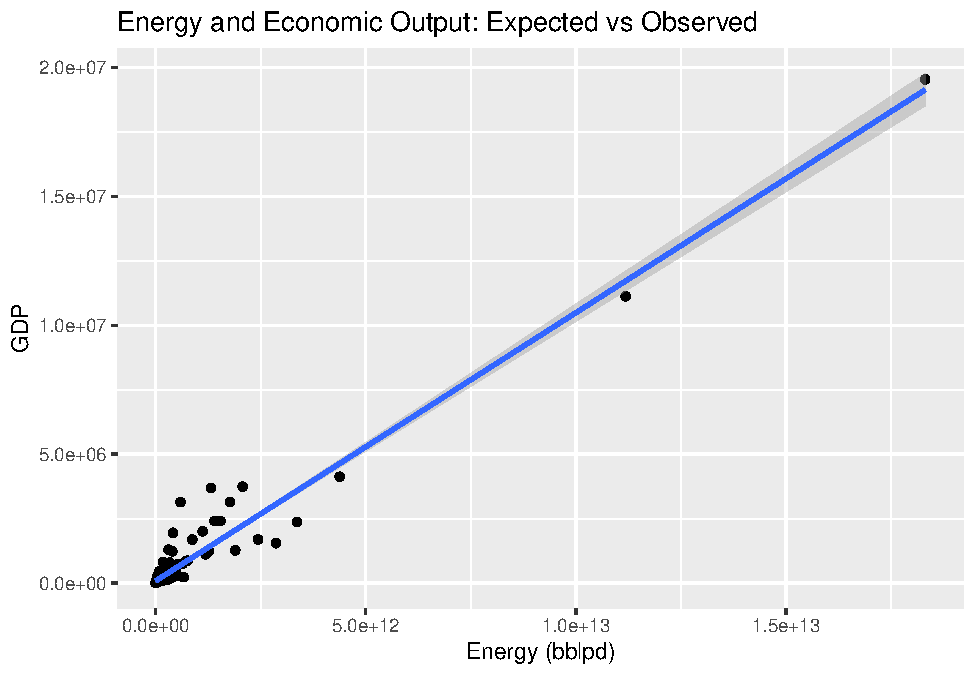
\includegraphics{Elsevier-Template_files/figure-latex/fig-energy-to-gdp-with-line-1.pdf}
\caption{\label{fig:energy-to-gdp-with-line} A regression line gives the
expected values of GDP given energy consumption}
\end{figure}

Figure \ref{fig:right-left-panel-plot} shows Figures
\ref{fig:energy-to-gdp} and \ref{fig:energy-to-gdp-with-line} side by
side.

\begin{figure}
\centering
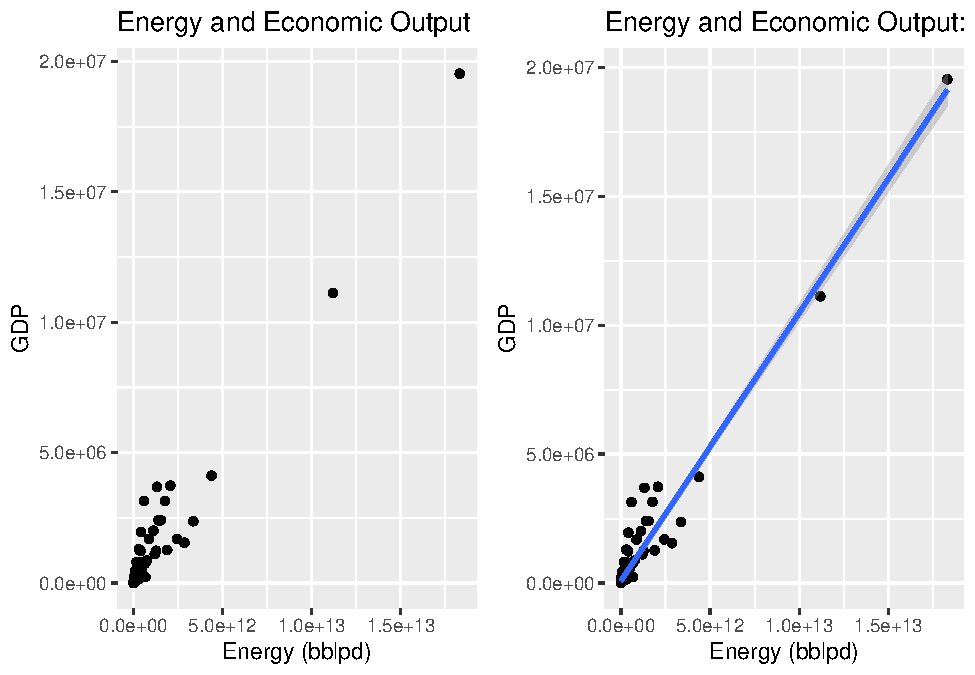
\includegraphics{Elsevier-Template_files/figure-latex/fig-right-left-panel-plot-1.pdf}
\caption{\label{fig:right-left-panel-plot} Two plots in a single figure;
left panel is Figure 1 and right panel is Figure 2}
\end{figure}

Figure \ref{fig:top-bottom-panel-plot} shows Figures
\ref{fig:energy-to-gdp} and \ref{fig:energy-to-gdp-with-line} as a
two-panel figure with one column and two rows.

\begin{figure}
\centering
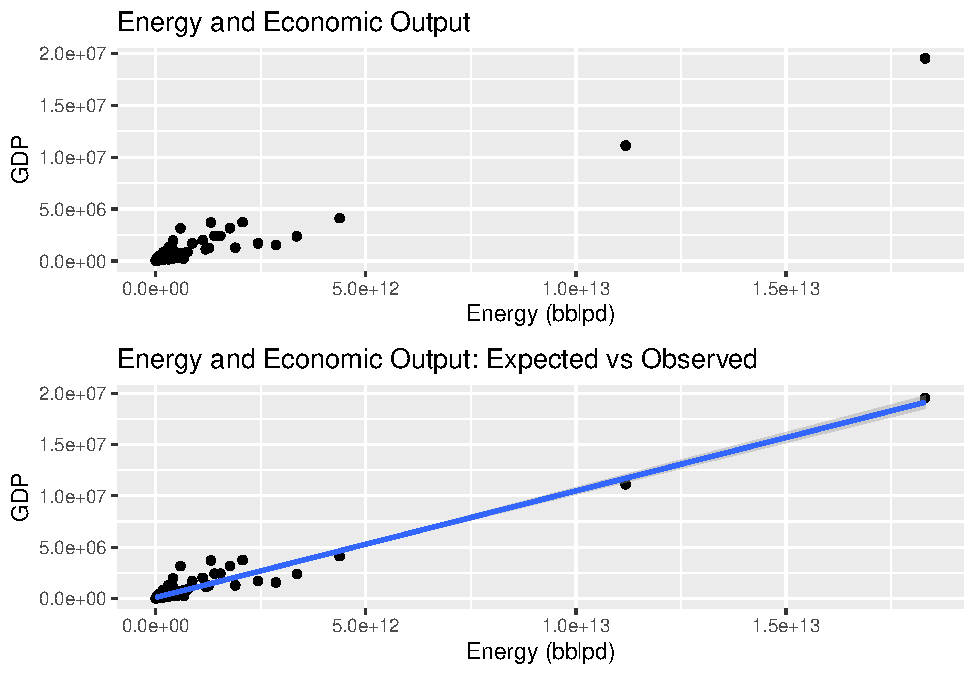
\includegraphics{Elsevier-Template_files/figure-latex/fig-top-bottom-panel-plot-1.pdf}
\caption{\label{fig:top-bottom-panel-plot} Two plots in a single figure;
top panel is Figure 1 and bottom panel is Figure 2}
\end{figure}

\begin{figure}
\centering
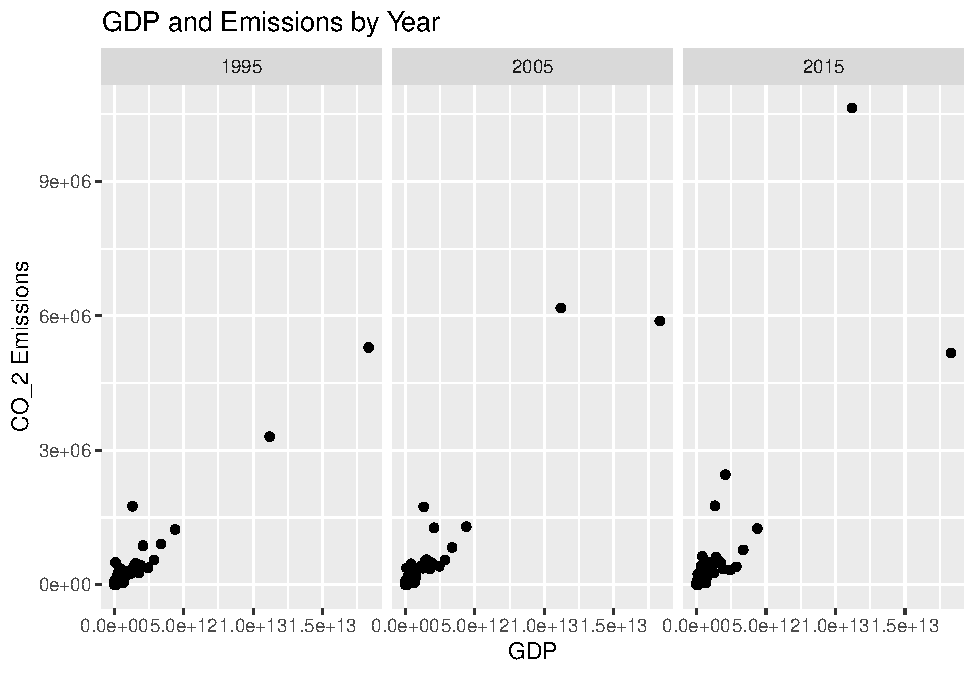
\includegraphics{Elsevier-Template_files/figure-latex/fig-gdp-emissions-by-year-1.pdf}
\caption{\label{fig:gdp-emissions-by-year} CO\_2 emissions versus GDP by
year}
\end{figure}

\hypertarget{methods}{%
\section{Methods}\label{methods}}

\hypertarget{spatial-autocorrelation-and-map-pattern}{%
\subsection{Spatial Autocorrelation and Map
Pattern}\label{spatial-autocorrelation-and-map-pattern}}

Spatial autocorrelation is a condition whereby the value of a variable
at one location is correlated with the value(s) of the same variable at
one or more proximal locations. A tool widely used to measure spatial
autocorrelation is Moran's coefficient of autocorrelation, or \(MC\) for
short. In matrix form, \(MC\) can be formulated as follows:

\begin{equation} 
\label{eq:1}
MC=\frac{n}{\sum_{i}{\sum_{j}{w_{ij}}}}\frac{x'Wx}{x'x}
\end{equation}

where \(x\) is a vector \((n\times1)\) of mean-centered values of a
georeferenced variable, and \(W\) is a spatial weights matrix of
dimensions \((n\times n)\) with elements \(w_{ij}\). The elements of the
spatial weights matrix take non-zero values if locations \(i\) and \(j\)
are deemed to be spatially proximate in some sense, and 0 otherwise. It
can be appreciated that the coefficient is composed to two elements: the
variance of the random variable (i.e., \((x' x)⁄n\)) and its spatial
autocovariance \(\frac{(x'Wx)}{\sum_{i}{\sum_{j}{w_{ij}}}}\). As an
alternative, the numerator of the right-hand term of Equation \ref{eq:1}
can be expressed as follows:

\begin{equation} 
\label{eq:2}
x'\Big(I - \frac{11'}{n}\Big)W\Big(I - \frac{11'}{n}\Big)x
\end{equation}

with \(I\) as the identity matrix of size \(n\times n\) and \(1\) a
conformable vector of ones.

One possible interpretation of spatial autocorrelation is as map
pattern. More concretely, the eigenvalues of the following matrix
represent the range of possible values of \(MC\) given a spatial weights
matrix \(W\), and the extreme eigenvalues are in fact associated with
the minimum and maximum values of \(MC\) for the system of relationships
represented by \(W\):

\begin{equation} 
\label{eq:3}
\Big(I - \frac{11'}{n}\Big)W\Big(I - \frac{11'}{n}\Big)
\end{equation}

A remarkable discovery is that the eigenvectors associated with the
eigenvalues of the matrix in Expression \ref{eq:3} represent a catalogue
of latent map patterns, each with a level of autocorrelation (as
measured by \(MC\)) given by its corresponding eigenvalue. Furthermore,
the patterns represented by the eigenvectors are orthogonal by design,
and so they furnish \(n\) maps that are independent from each other.
Since these map patterns depend only on the spatial weights matrix --
and not the spatial random variable -- they constitute an extensive set
of latent map patterns that can be used in regression analysis as
filters. This is explained next.

\hypertarget{references}{%
\section*{References}\label{references}}
\addcontentsline{toc}{section}{References}


\end{document}


